%\subsection{Portfolio f\"ur Research Object und Evaluation Methods (Gr\"o\ss{}e entspricht der Anzahl)}
%\begin{figure}
\begin{center}
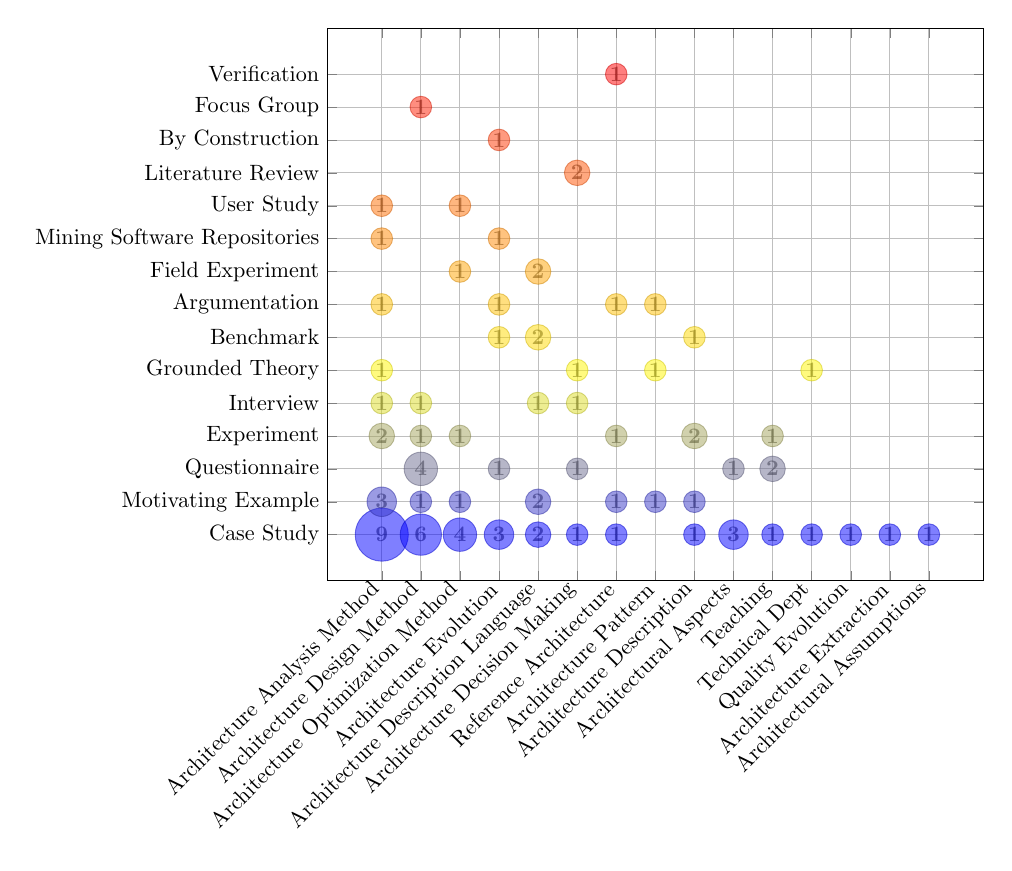
\begin{tikzpicture}[scale=.8]
\begin{axis}[scatter,
    width=.99\linewidth,
    cycle multi list=Spectral,
    every axis plot/.append style={draw, fill, fill opacity=0.5},
    scatter src=y,
    nodes near coords style={color=black,font=\small},
    %enlargelimits=0.15,
    x tick label style={rotate=45,anchor=east},
    xtick={0,1,2,3,4,5,6,7,8,9,10,11,12,13,14}, xticklabels={Architecture Analysis Method,Architecture Design Method,Architecture Optimization Method,Architecture Evolution,Architecture Description Language,Architecture Decision Making,Reference Architecture,Architecture Pattern,Architecture Description,Architectural Aspects,Teaching,Technical Dept,Quality Evolution,Architecture Extraction,Architectural Assumptions},
    ytick={0,1,2,3,4,5,6,7,8,9,10,11,12,13,14}, yticklabels={Case Study,Motivating Example,Questionnaire,Experiment,Interview,Grounded Theory,Benchmark,Argumentation,Field Experiment,Mining Software Repositories,User Study,Literature Review,By Construction,Focus Group,Verification},
    grid=both
]

\addplot[mark size=12.000,opacity=0.5,text=black] coordinates { (0,0) } node[text=black,font=\bfseries] {9};
\addplot[mark size=6.667,opacity=0.5,text=black] coordinates { (0,1) } node[text=black,font=\bfseries] {3};
\addplot[mark size=5.778,opacity=0.5,text=black] coordinates { (0,3) } node[text=black,font=\bfseries] {2};
\addplot[mark size=4.889,opacity=0.5,text=black] coordinates { (0,4) } node[text=black,font=\bfseries] {1};
\addplot[mark size=4.889,opacity=0.5,text=black] coordinates { (0,5) } node[text=black,font=\bfseries] {1};
\addplot[mark size=4.889,opacity=0.5,text=black] coordinates { (0,7) } node[text=black,font=\bfseries] {1};
\addplot[mark size=4.889,opacity=0.5,text=black] coordinates { (0,9) } node[text=black,font=\bfseries] {1};
\addplot[mark size=4.889,opacity=0.5,text=black] coordinates { (0,10) } node[text=black,font=\bfseries] {1};
\addplot[mark size=9.333,opacity=0.5,text=black] coordinates { (1,0) } node[text=black,font=\bfseries] {6};
\addplot[mark size=4.889,opacity=0.5,text=black] coordinates { (1,1) } node[text=black,font=\bfseries] {1};
\addplot[mark size=7.556,opacity=0.5,text=black] coordinates { (1,2) } node[text=black,font=\bfseries] {4};
\addplot[mark size=4.889,opacity=0.5,text=black] coordinates { (1,3) } node[text=black,font=\bfseries] {1};
\addplot[mark size=4.889,opacity=0.5,text=black] coordinates { (1,4) } node[text=black,font=\bfseries] {1};
\addplot[mark size=4.889,opacity=0.5,text=black] coordinates { (1,13) } node[text=black,font=\bfseries] {1};
\addplot[mark size=7.556,opacity=0.5,text=black] coordinates { (2,0) } node[text=black,font=\bfseries] {4};
\addplot[mark size=4.889,opacity=0.5,text=black] coordinates { (2,1) } node[text=black,font=\bfseries] {1};
\addplot[mark size=4.889,opacity=0.5,text=black] coordinates { (2,3) } node[text=black,font=\bfseries] {1};
\addplot[mark size=4.889,opacity=0.5,text=black] coordinates { (2,8) } node[text=black,font=\bfseries] {1};
\addplot[mark size=4.889,opacity=0.5,text=black] coordinates { (2,10) } node[text=black,font=\bfseries] {1};
\addplot[mark size=6.667,opacity=0.5,text=black] coordinates { (3,0) } node[text=black,font=\bfseries] {3};
\addplot[mark size=4.889,opacity=0.5,text=black] coordinates { (3,2) } node[text=black,font=\bfseries] {1};
\addplot[mark size=4.889,opacity=0.5,text=black] coordinates { (3,6) } node[text=black,font=\bfseries] {1};
\addplot[mark size=4.889,opacity=0.5,text=black] coordinates { (3,7) } node[text=black,font=\bfseries] {1};
\addplot[mark size=4.889,opacity=0.5,text=black] coordinates { (3,9) } node[text=black,font=\bfseries] {1};
\addplot[mark size=4.889,opacity=0.5,text=black] coordinates { (3,12) } node[text=black,font=\bfseries] {1};
\addplot[mark size=5.778,opacity=0.5,text=black] coordinates { (4,0) } node[text=black,font=\bfseries] {2};
\addplot[mark size=5.778,opacity=0.5,text=black] coordinates { (4,1) } node[text=black,font=\bfseries] {2};
\addplot[mark size=4.889,opacity=0.5,text=black] coordinates { (4,4) } node[text=black,font=\bfseries] {1};
\addplot[mark size=5.778,opacity=0.5,text=black] coordinates { (4,6) } node[text=black,font=\bfseries] {2};
\addplot[mark size=5.778,opacity=0.5,text=black] coordinates { (4,8) } node[text=black,font=\bfseries] {2};
\addplot[mark size=4.889,opacity=0.5,text=black] coordinates { (5,0) } node[text=black,font=\bfseries] {1};
\addplot[mark size=4.889,opacity=0.5,text=black] coordinates { (5,2) } node[text=black,font=\bfseries] {1};
\addplot[mark size=4.889,opacity=0.5,text=black] coordinates { (5,4) } node[text=black,font=\bfseries] {1};
\addplot[mark size=4.889,opacity=0.5,text=black] coordinates { (5,5) } node[text=black,font=\bfseries] {1};
\addplot[mark size=5.778,opacity=0.5,text=black] coordinates { (5,11) } node[text=black,font=\bfseries] {2};
\addplot[mark size=4.889,opacity=0.5,text=black] coordinates { (6,0) } node[text=black,font=\bfseries] {1};
\addplot[mark size=4.889,opacity=0.5,text=black] coordinates { (6,1) } node[text=black,font=\bfseries] {1};
\addplot[mark size=4.889,opacity=0.5,text=black] coordinates { (6,3) } node[text=black,font=\bfseries] {1};
\addplot[mark size=4.889,opacity=0.5,text=black] coordinates { (6,7) } node[text=black,font=\bfseries] {1};
\addplot[mark size=4.889,opacity=0.5,text=black] coordinates { (6,14) } node[text=black,font=\bfseries] {1};
\addplot[mark size=4.889,opacity=0.5,text=black] coordinates { (7,1) } node[text=black,font=\bfseries] {1};
\addplot[mark size=4.889,opacity=0.5,text=black] coordinates { (7,5) } node[text=black,font=\bfseries] {1};
\addplot[mark size=4.889,opacity=0.5,text=black] coordinates { (7,7) } node[text=black,font=\bfseries] {1};
\addplot[mark size=4.889,opacity=0.5,text=black] coordinates { (8,0) } node[text=black,font=\bfseries] {1};
\addplot[mark size=4.889,opacity=0.5,text=black] coordinates { (8,1) } node[text=black,font=\bfseries] {1};
\addplot[mark size=5.778,opacity=0.5,text=black] coordinates { (8,3) } node[text=black,font=\bfseries] {2};
\addplot[mark size=4.889,opacity=0.5,text=black] coordinates { (8,6) } node[text=black,font=\bfseries] {1};
\addplot[mark size=6.667,opacity=0.5,text=black] coordinates { (9,0) } node[text=black,font=\bfseries] {3};
\addplot[mark size=4.889,opacity=0.5,text=black] coordinates { (9,2) } node[text=black,font=\bfseries] {1};
\addplot[mark size=4.889,opacity=0.5,text=black] coordinates { (10,0) } node[text=black,font=\bfseries] {1};
\addplot[mark size=5.778,opacity=0.5,text=black] coordinates { (10,2) } node[text=black,font=\bfseries] {2};
\addplot[mark size=4.889,opacity=0.5,text=black] coordinates { (10,3) } node[text=black,font=\bfseries] {1};
\addplot[mark size=4.889,opacity=0.5,text=black] coordinates { (11,0) } node[text=black,font=\bfseries] {1};
\addplot[mark size=4.889,opacity=0.5,text=black] coordinates { (11,5) } node[text=black,font=\bfseries] {1};
\addplot[mark size=4.889,opacity=0.5,text=black] coordinates { (12,0) } node[text=black,font=\bfseries] {1};
\addplot[mark size=4.889,opacity=0.5,text=black] coordinates { (13,0) } node[text=black,font=\bfseries] {1};
\addplot[mark size=4.889,opacity=0.5,text=black] coordinates { (14,0) } node[text=black,font=\bfseries] {1};


\end{axis}
\end{tikzpicture}
\end{center}
%\caption{Portfolio f\"ur Research Object und Evaluation Methods (Gr\"o\ss{}e entspricht der Anzahl)}\label{fig:port_researchobject_evaluationmethods}
%\end{figure}

